\documentclass[aspectratio=169]{beamer}
\usetheme{Madrid}
\usecolortheme{default}

% Packages
\usepackage{graphicx}
\usepackage{amsmath}
\usepackage{booktabs}
\usepackage{tikz}

% Custom colors
\definecolor{darkgreen}{RGB}{34,139,34}
\definecolor{darkblue}{RGB}{0,51,102}

\title{Pass Decision Making in Soccer: An MDP Approach}
\subtitle{Extending Van Roy et al.'s Leaving Goals on the Pitch: Evaluating Decision Making in Soccer}
\author{Martim Rêgo}
\institute{Deep Learning \& AI in Sport}
\date{November 2025}

\begin{document}

% Title slide
\frame{\titlepage}

% ============================================
% SECTION 1: Reference Paper Overview (1 min)
% ============================================
\section{Reference Paper}

\begin{frame}{Van Roy et al. (2020): "Leaving Goals on the Pitch"}
\begin{columns}[T]
\column{0.45\textwidth}
\textbf{Setup:}
\begin{itemize}
    \item EPL 2017-19
    \item \textbf{Question:} Shoot from distance or pass?
    \item 22×17 grid (374 states)
    \item Actions: Move or shoot
\end{itemize}

\vspace{0.2cm}
\textbf{MDP Components:}
\begin{itemize}
    \item \textbf{States:} Field zones
    \item \textbf{Actions:} Move/shoot
    \item \textbf{Transitions:} $P(s'|s,a)$
    \item \textbf{Policy:} $\pi(a|s)$
    \item \textbf{Rewards:} Goals
\end{itemize}

\column{0.55\textwidth}
\vspace{-0.3cm}
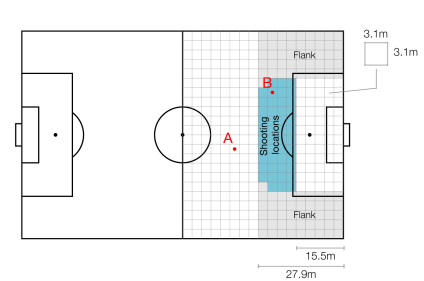
\includegraphics[width=0.85\textwidth]{outputs/figures/paper_states.png}

\vspace{0.1cm}
\textbf{Key Findings:}
\begin{itemize}
    \item Teams shoot \textbf{too rarely} from distance
    \item 10-20\% more long shots → +1 goal/season
    \item Specific zones: shooting $>$ passing
\end{itemize}
\end{columns}
\end{frame}

% ============================================
% SECTION 2: Our Approach (1.5 min)
% ============================================
\section{Our Approach}

\begin{frame}{Our Extension: Pass Decision Analysis}
\begin{columns}[T]
\column{0.5\textwidth}
\textbf{What We Changed:}
\begin{itemize}
    \item[\checkmark] Action space: 8 actions
    \begin{itemize}
        \item 6 pass types (length × direction)
        \item Shoot
        \item Carry (dribbling)
    \end{itemize}
    \item[\checkmark] Grid: 7×11 (77 states) — simplified
    \item[\checkmark] Data: Premier League 2024/25 (521K actions)
    \item[\checkmark] Action masking for physical constraints
\end{itemize}

\column{0.5\textwidth}
\textbf{Pass Classification:}
\begin{itemize}
    \item \textbf{Length:} Short ($\leq$25m) vs Long ($>$25m)
    \item \textbf{Direction:} Forward / Lateral / Backward
    \begin{itemize}
        \item Angle-based
    \end{itemize}
\end{itemize}

\vspace{0.3cm}
\textbf{Action Masking:}
\begin{itemize}
    \item Shooting: disabled $>$30m from goal
    \item Long forward: disabled near goal
    \item Long backward: disabled near own goal
\end{itemize}
\end{columns}
\end{frame}

\begin{frame}{Dataset Overview}
\begin{columns}[T]
\column{0.5\textwidth}
\textbf{Data Volume:}
\begin{itemize}
    \item 378 matches (PL 2024/25 season)
    \item 521,470 total actions
    \begin{itemize}
        \item 328,713 passes (63.0\%)
        \item 184,080 carries (35.3\%)
        \item 8,677 shots (1.7\%)
    \end{itemize}
    \item 20 teams analyzed
\end{itemize}

\column{0.5\textwidth}
\textbf{Success Rates:}
\begin{itemize}
    \item Passes: 82.85\%
    \item Shots (goals): 12.3\%
    \item Carries: 91.6\%
\end{itemize}

\vspace{0.3cm}
\textbf{State-Action Coverage:}
\begin{itemize}
    \item 579 unique (s, a) pairs observed
    \item 94\% coverage (excellent!)
    \item Mean: 900.6 obs/pair
\end{itemize}
\end{columns}
\end{frame}

\begin{frame}{MDP Construction}
\begin{columns}[T]
\column{0.5\textwidth}
\textbf{For Each Team:}
\begin{enumerate}
    \item \textbf{Transition Matrix $P$}
    \begin{itemize}
        \item Shape: (80, 8, 80)
        \item 77 field + 3 absorbing states
        \item \textbf{Learned from data:}
        \begin{itemize}
            \item Passes/carries: Laplace smoothing ($\alpha = 2.0$)
            \item Shots: Bayesian shrinkage ($\alpha = 10$)
        \end{itemize}
    \end{itemize}
    
    \item \textbf{Policy Matrix $\pi$}
    \begin{itemize}
        \item Shape: (77, 8)
        \item Observed action frequencies
    \end{itemize}
    
    \item \textbf{Reward Vector $R$}
    \begin{itemize}
        \item R(goal) = 1, else 0
    \end{itemize}
\end{enumerate}

\column{0.5\textwidth}
\textbf{Absorbing States:}
\begin{itemize}
    \item State 77: Goal (successful shot)
    \item State 78: No goal (failed shot)
    \item State 79: Loss of possession
\end{itemize}

\vspace{0.3cm}
\textbf{Position-Based xG:}
\begin{itemize}
    \item Geometric model: viewing angle to goal
    \item $xG = 0.76 \times \left(\frac{\theta}{36.8^{\circ}}\right)^{1.5}$
    \item Used for shot transitions
\end{itemize}
\end{columns}
\end{frame}

\begin{frame}{Fundamental Matrix: Theoretical Foundation}
\begin{columns}[T]
\column{0.55\textwidth}
\textbf{Definition:}
$$\mathbf{N} = (\mathbf{I} - \mathbf{Q})^{-1}$$

where $\mathbf{Q}$ contains transition probabilities between transient (field) states.

\vspace{0.2cm}
\textbf{Interpretation:}
\begin{itemize}
    \item $N_{ij}$ = expected visits to state $j$ from state $i$
    \item Captures \textbf{all possible paths} before absorption
    \item Multi-step sequences handled automatically
\end{itemize}

\column{0.45\textwidth}
\textbf{Computing Expected Goals:}
$$E[\text{goals} | s_0] = \sum_{j} N_{s_0,j} \cdot \pi(\text{shoot} | j) \cdot xG(j)$$

\vspace{0.2cm}
\textbf{Why It's Powerful:}
\begin{itemize}
    \item Exact calculation (no simulation)
    \item Handles uncertainty
    \item Enables counterfactual reasoning
    \item Foundation for policy evaluation
\end{itemize}
\end{columns}
\end{frame}

\begin{frame}{Computed Expected Goals per Team for the whole season}
\begin{center}
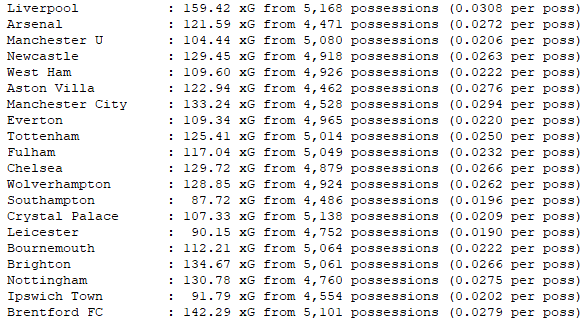
\includegraphics[width=0.8\textwidth]{outputs/figures/xg_per_team.png}
\end{center}

\vspace{0.3cm}
\begin{columns}[T]
\column{0.5\textwidth}
\textbf{Top Teams (Expected Goals):}
\begin{enumerate}
    \item Man City: 136.5 xG
    \item Liverpool: 128.3 xG
    \item Arsenal: 121.7 xG
\end{enumerate}

\column{0.5\textwidth}
\textbf{Key Metrics:}
\begin{itemize}
    \item League avg: 123.1 xG
    \item Range: 98-137 xG
    \item Possession \% $\neq$ Expected goals
    \item Directness matters!
\end{itemize}
\end{columns}

\vspace{0.3cm}
\begin{block}{Insight}
Even top teams leave goals on the pitch by not optimizing pass decisions in key zones
\end{block}
\end{frame}

% ============================================
% SECTION 3: Results (2 min)
% ============================================
\section{Results}

\begin{frame}{Result 1: Optimal Action Selection}
\textbf{Research Question:} Which action maximizes goal probability from each zone?

\vspace{0.3cm}
\begin{center}
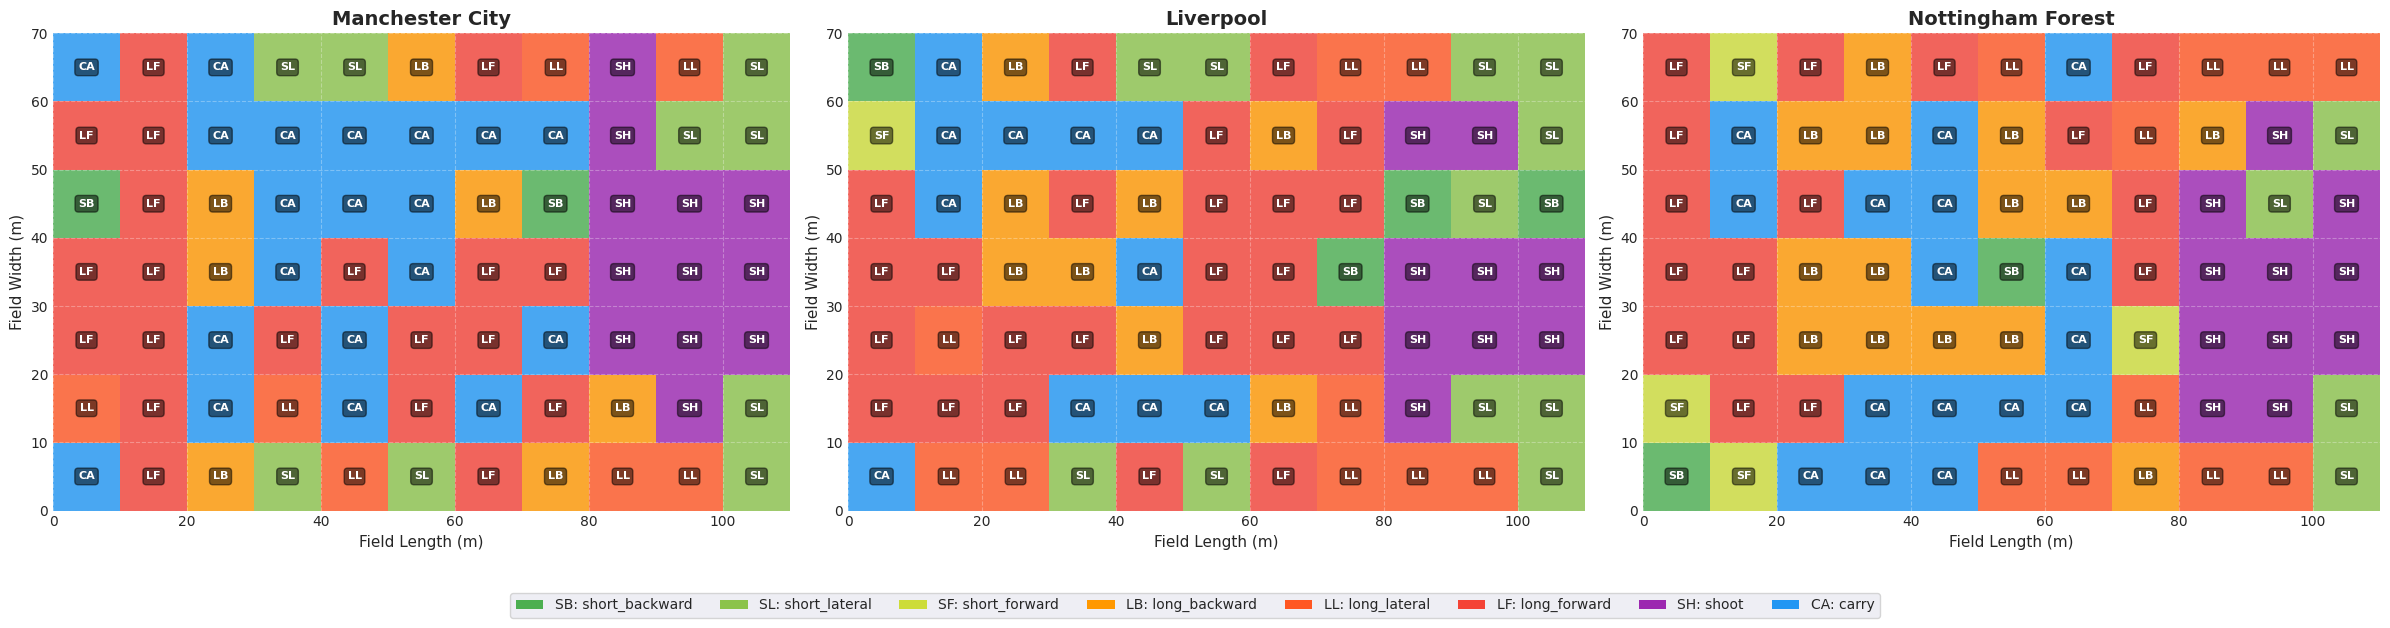
\includegraphics[width=\textwidth,height=0.9\textheight,keepaspectratio]{outputs/figures/optimal_actions.png}
\end{center}
\end{frame}

\begin{frame}{Result 2: Quality-Quantity Trade-Offs}
\vspace{-0.1cm}
\textbf{Critical Insight:} Increasing action frequency reduces success rates

\vspace{0.2cm}
\begin{center}
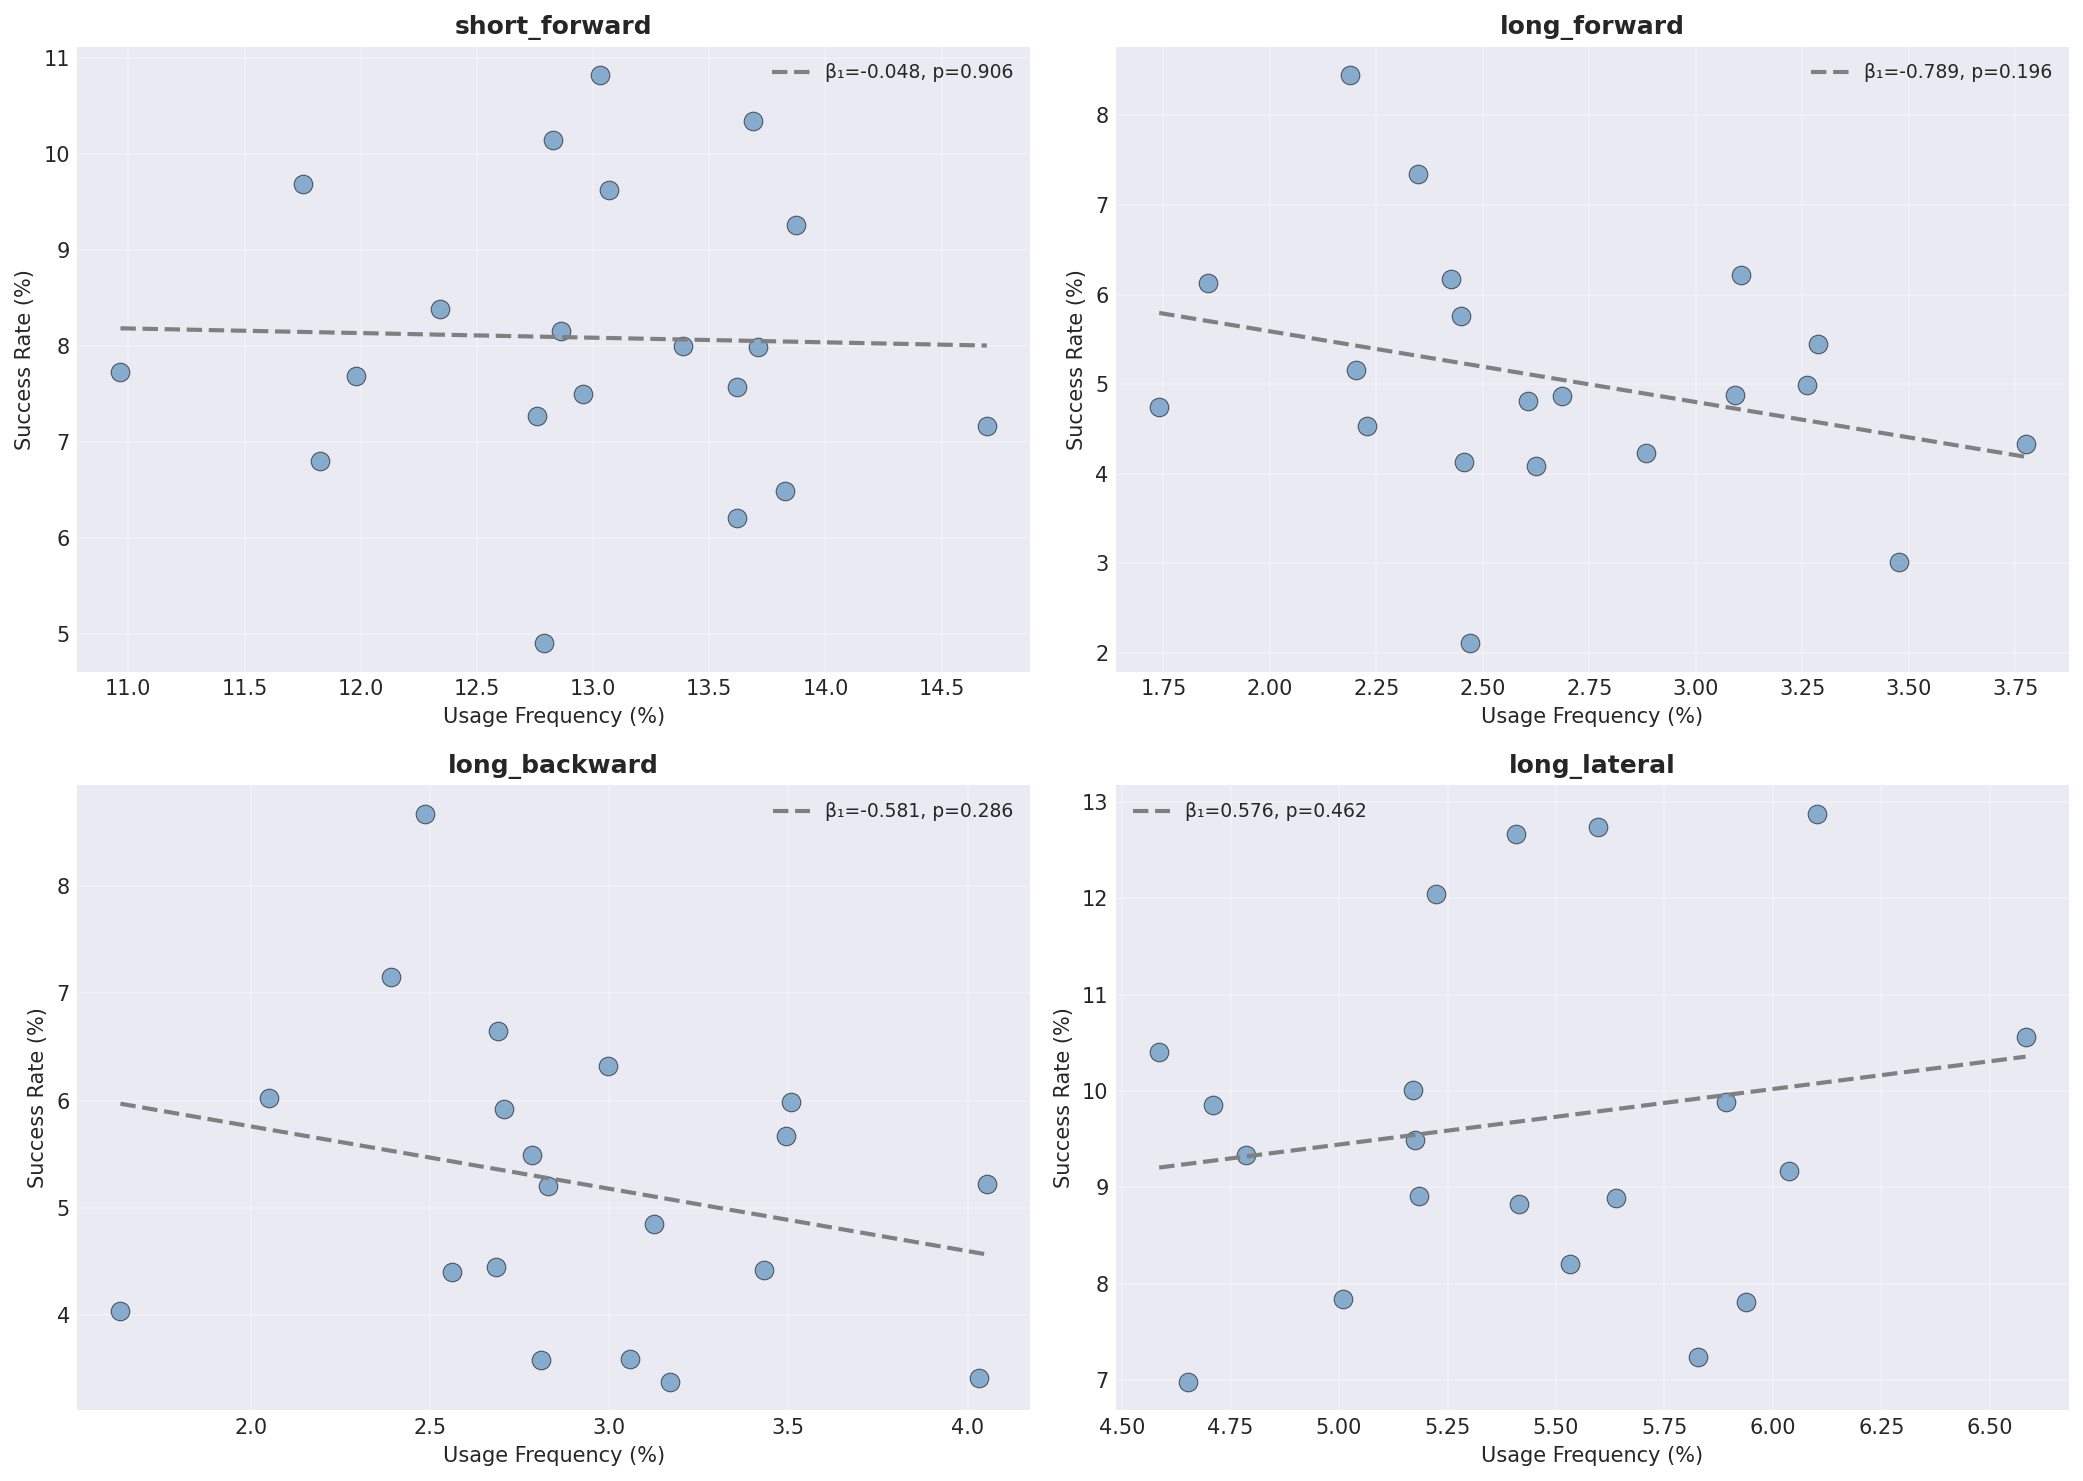
\includegraphics[width=0.6\textwidth]{outputs/figures/quality_quantity_tradeoffs.png}
\end{center}

\end{frame}

\begin{frame}{Result 3: Counterfactual Policy Analysis}
\textbf{Research Question:} What if teams altered their pass policies?

\vspace{0.3cm}
\begin{center}
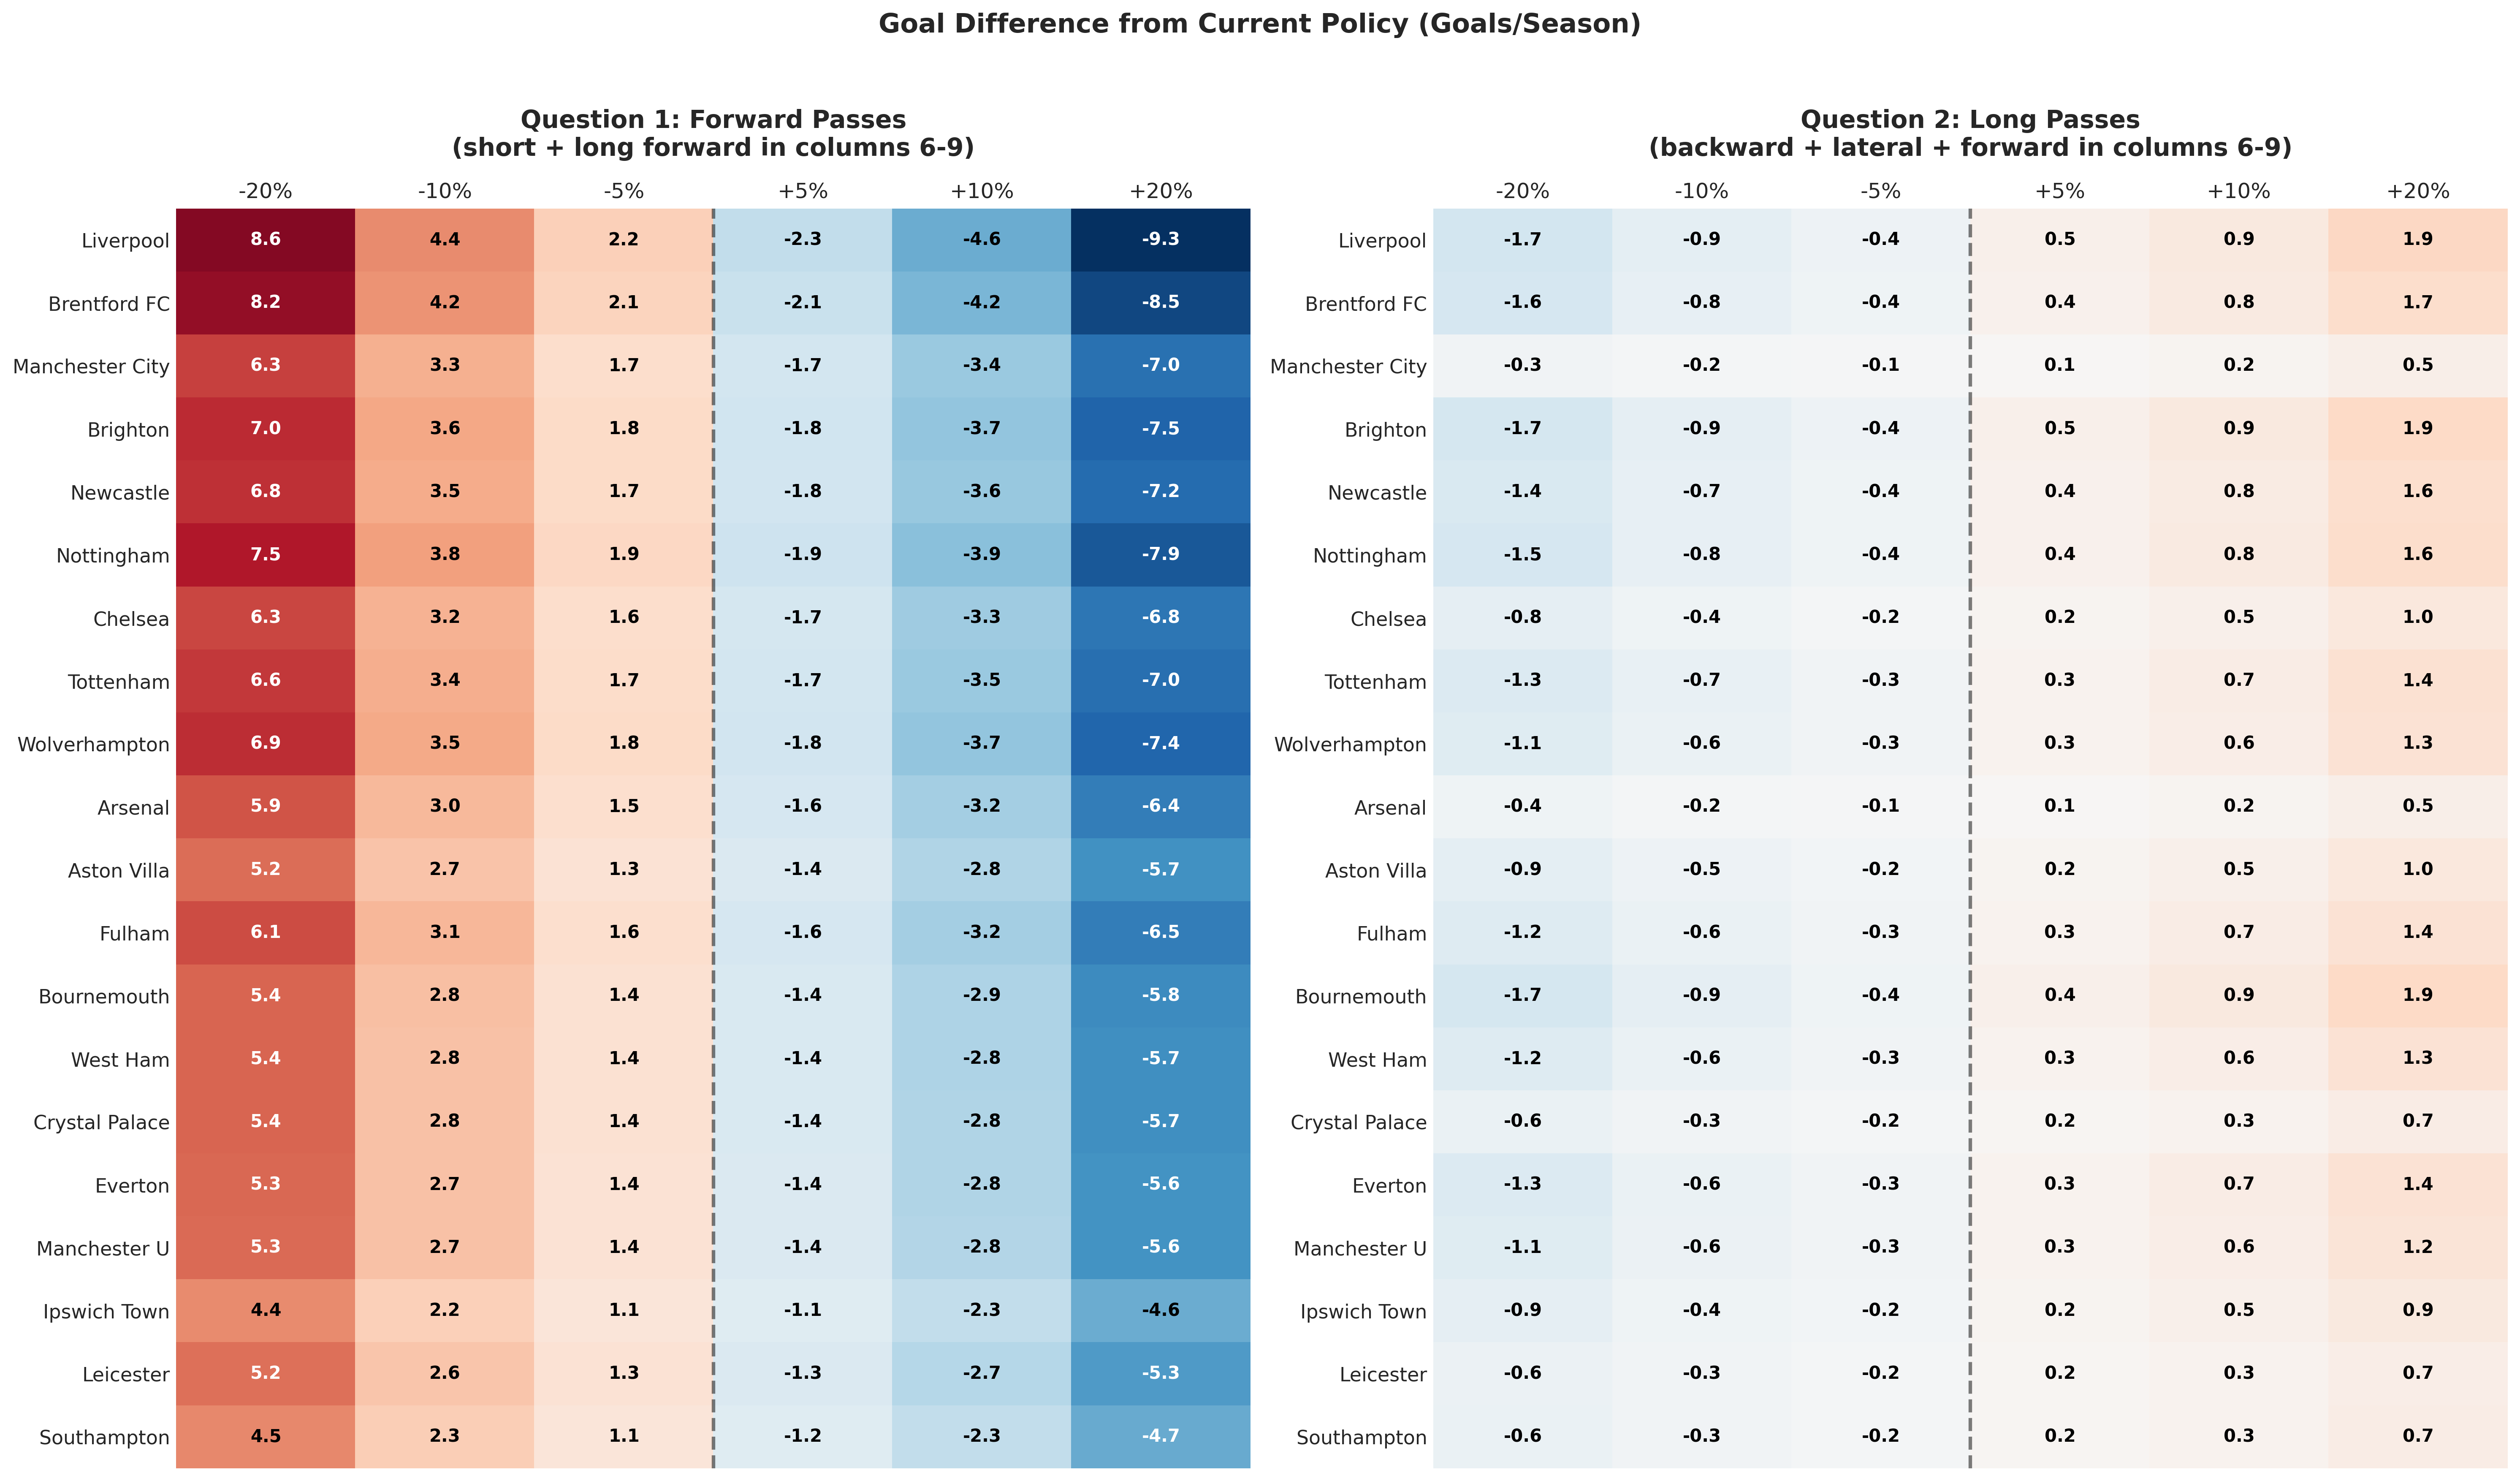
\includegraphics[width=0.7\textwidth]{outputs/figures/counterfactual_vanroy_style.png}
\end{center}

\end{frame}

\begin{frame}{Result 4: Directness vs. Patient Build-Up}
\textbf{Research Question:} 1 long forward pass vs 2 short forward passes in attacking half?

\vspace{0.3cm}
\begin{center}
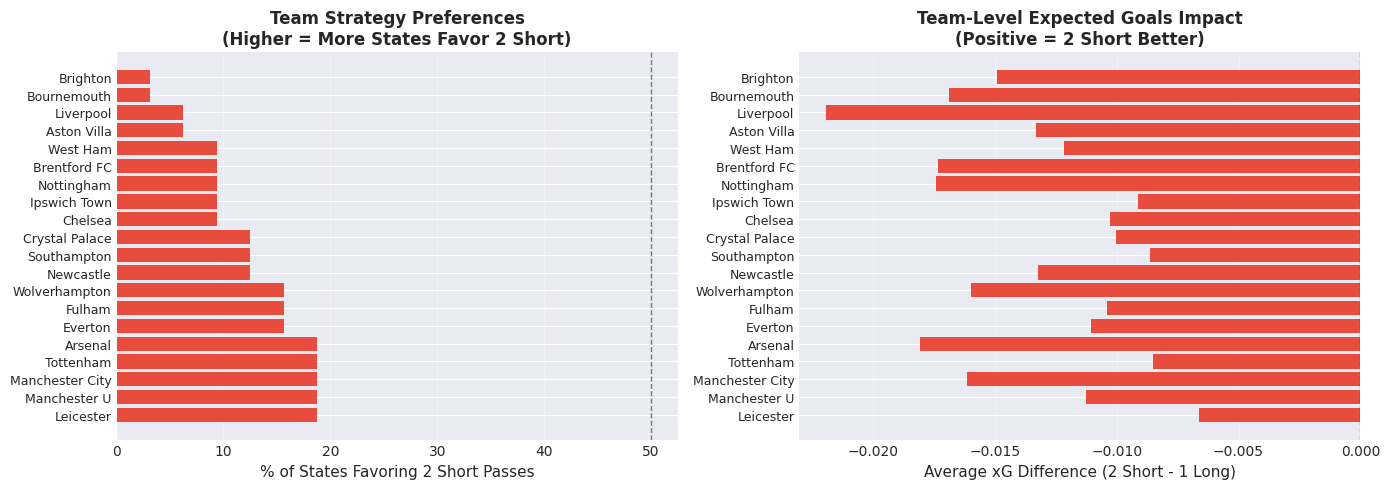
\includegraphics[width=0.75\textwidth]{outputs/figures/short_long_all.png}
\end{center}

\vspace{0.3cm}
\textbf{Key Findings (Monte Carlo simulation, 3000 runs):}
\begin{itemize}
    \item \textbf{All 20 teams} benefit from directness in 80-97\% of valid positions
    \item League average: \textbf{+0.0132 xG} for 1 long forward pass
    \item Result holds across all playing styles
    \item \textbf{Masked zones:} Long forward passes disabled in columns 9-10 (attacking zone)
\end{itemize}

\vspace{0.2cm}
\begin{center}
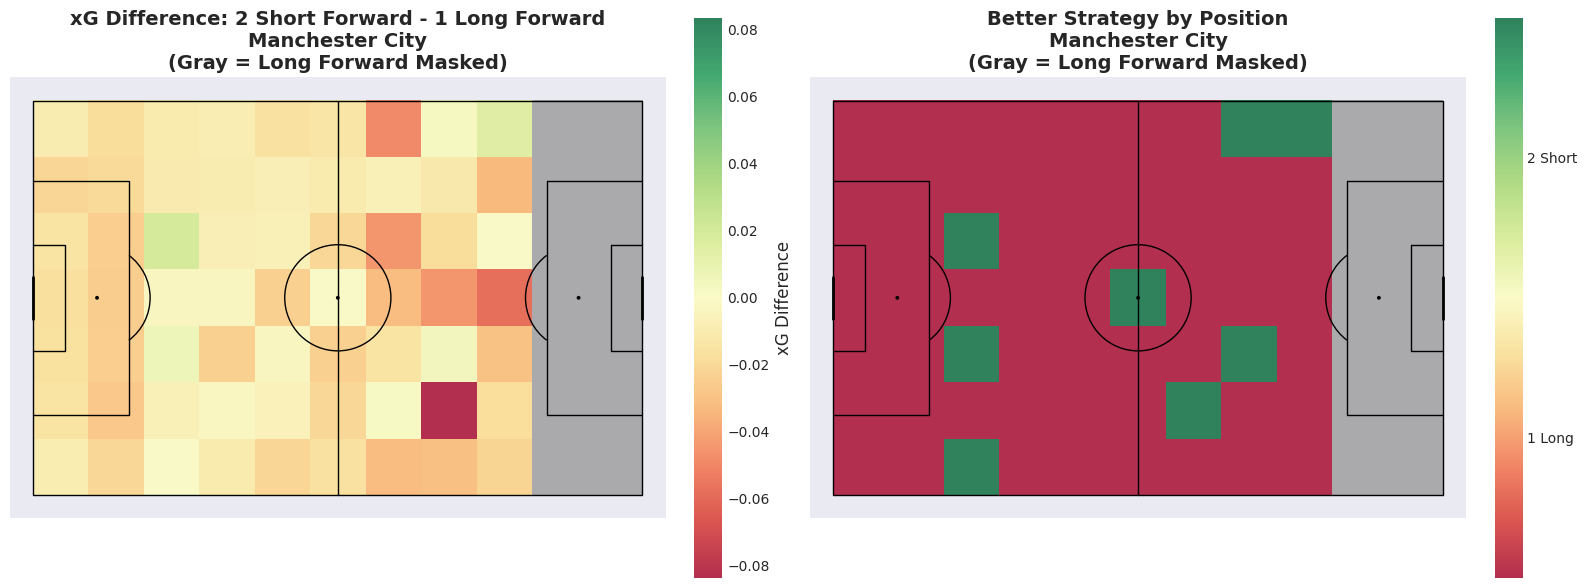
\includegraphics[width=0.6\textwidth]{outputs/figures/short_long_city.png}
\end{center}
\end{frame}

% ============================================
% SECTION 4: Conclusion (0.5 min)
% ============================================
\section{Conclusion}

\begin{frame}{Summary \& Contributions}
\begin{columns}[T]
\column{0.5\textwidth}
\textbf{What We Did:}
\begin{enumerate}
    \item Extended Van Roy's shooting MDP to \textbf{pass policy analysis}
    \item Monte Carlo simulation for strategy comparison
    \item Otherwise similar methodology
\end{enumerate}

\column{0.5\textwidth}
\textbf{Key Findings:}
\begin{itemize}
    \item Teams benefit from longer passes
    \item Teams benefit from less forward passes
    \item Team-specific optimal policies
\end{itemize}
\end{columns}

\vspace{0.5cm}
\textbf{Practical Applications:}
\begin{itemize}
    \item Tactical coaching: Which zones favor long vs short passes?
    \item Match preparation: Opponent analysis
    \item Recruitment: Identify decision-making quality
\end{itemize}
\end{frame}

\begin{frame}{Limitations \& Future Work}
\begin{columns}[T]
\column{0.5\textwidth}
\textbf{Limitations:}
\begin{itemize}
    \item Grid discretization (7×11) loses detail
    \item Markov property assumption
    \item No opponent modeling
    \item Absolute xG values overestimated
\end{itemize}

\column{0.5\textwidth}
\textbf{Future Work:}
\begin{itemize}
    \item Finer grid resolution
    \item Player-level policies
    \item Opponent modeling
\end{itemize}
\end{columns}

\vspace{0.5cm}
\begin{center}
\Large \textbf{Thank You!}

\vspace{0.3cm}
\normalsize Questions?
\end{center}
\end{frame}

\end{document}
